\section{Summary}\label{summary}

\texttt{hashin\_shtrikman\_mp} is a tool for composites designers who
have desired composite properties in mind, but who do not yet have an
underlying formulation. The library utilizes the tightest theoretical
bounds on the effective properties of composite materials with
unspecified microstructure -- the Hashin-Shtrikman bounds -- to identify
candidate theoretical materials, find real materials that are close to
the candidates, and determine the optimal volume fractions for each of
the constituents in the resulting composite. Its i) leveraging of
materials in the \href{https://next-gen.materialsproject.org/}{Materials
Project} database, ii) integration with the
\href{https://next-gen.materialsproject.org/api}{Materials Project API},
iii) use of genetic machine-learning and iv) agnosticism to underlying
microstructure, and v) ultimate engineering application, make it a tool
with much broader applications than its predecessors.

\section{Statement of need}\label{statement-of-need}

Composites are ubiquitous in engineering due to their tunability and
enhanced material properties as compared to their individual
constituents. As such, composite design is an active field, but the
pursuit of new materials through experimentation is expensive. Today,
computational tools for materials design are integral to reducing the
cost and increasing the pace of innovation in sectors like energy,
electronics, aviation and beyond.

Several Python packages already exist for specific areas in composites
modeling, such as \href{https://github.com/Extraweich/homopy}{HomoPy},
\href{https://github.com/rafaelcidade/compositeslib}{CompositesLib},
\href{https://github.com/echaffey/Compysite}{Compysite},
\href{https://github.com/azzeddinetiba/FeCLAP}{FeCLAP}, and
\href{https://pypi.org/project/material-mechanics/}{material-mechanics},
all of which perform stress analysis on laminates and/or
fiber-reinforced composites using either classical laminate theory or
the finite element method. Others exist which, like
\texttt{hashin\_shtrikman\_mp}, utilize the Hashin-Shtrikman bounds on
effective composite properties, such as
\href{https://geodynamics.github.io/burnman/}{BurnMan} for thermal
analysis of composite rocks/assemblages,
\href{https://rockphypy.readthedocs.io/en/latest/getting_started/08_Shaly_sand_modelling.html}{rockphypy}
for mechanical modeling of sand-shale systems, {[}@ZARE2017176{]}'s
modeling of clay nanocomposites,
\href{https://github.com/JulianKarlBauer/mechmean/tree/main?tab=readme-ov-file}{mechmean},
and {[}@ZERHOUNI2019344{]}'s modeling of 3D printed microstructures. All
of these tools, however, are highly specific to composite
microstructure, macro-geometry, and composition. More notably, they
focus on analysis of already well-defined composites, rather than
discovery of new materials.

\texttt{hashin\_shtrikman\_mp} is intended for composites designers who
are much earlier in their design process -- designers who are seeking
out new composite formulations and who are not yet tied to a specific
underlying microstructure. \texttt{hashin\_shtrikman\_mp} defines an
inverse problem wherein composite formulations which achieve a desired
behavior are found by minimizing a cost function
{[}@zohdi2012electromagnetic{]}. Accounting for both absolute error from
the desired properties and targeting even load distribution across
constituent phases, \texttt{hashin\_shtrikman\_mp} returns candidate
theoretical materials, then searches for real materials in the Materials
Project database with properties close to the recommended constituents.

\section{Underlying theory}\label{underlying-theory}

\subsection{Estimate effective composite properties with the
Hashin-Shtrikman
bounds}\label{estimate-effective-composite-properties-with-the-hashin-shtrikman-bounds}

When designing composites, simple volume-weighted linear combinations of
constituent material properties do not yield accurate approximations of
the resulting effective composite properties. Instead, for laminates,
materials designers often bound the resulting composite properties using
equations from constitutive elastic theory, such as the
Hill-Reuss-Voight-Weiner bounds, where the lower bound is the harmonic
mean of the constituent material properties and the upper bound is the
arithmetic mean {[}@commentaryHS{]}. For quasi-isotropic and
quasi-homogeneous multi-phase composites with arbitrary phase geometry
(a more general case), a better option is to use the Hashin-Shtrikman
bounds, which provide even tighter ranges on the resulting effective
properties {[}@hashin1962variational{]}. \autoref{eqn:gen_ineq}
summarizes the Hashin-Shtrikman bounds on a generalized effective
material property \(y^{*}\) of an \(n\)-phase composite. The generalized
material properties for the \(n\)-phases are ordered from least to
greatest where \(y_{1} \leq y_{2} \leq \dotsb \leq y_{n}\) with
corresponding volume fractions that sum to unity
\(v_{1} + v_{2} + \dotsb + v_{n} = 1\), and are given by

\begin{equation}\label{eqn:gen_ineq}
y_{1} + \frac{A_{1}}{1 - \alpha_{1}A_{1}}
= y^{*,-} \leq y^{*} \leq y^{*,+} = 
y_{n} + \frac{A_{n}}{1 - \alpha_{n}A_{n}}
\end{equation}

where \begin{equation}\label{eqn:gen_alphas}
\alpha_{1} = \frac{1}{3y_{1}}
\quad \text{and} \quad
\alpha_{n} = \frac{1}{3y_{n}},
\end{equation}

and \begin{equation}\label{eqn:gen_As}
A_{1} = \sum\limits_{i=2}^{n} \frac{v_{i}}{\frac{1}{y_{i} - y_{1}} + \alpha_{1}}
\quad \text{and} \quad
A_{n} = \sum\limits_{i=1}^{n-1} \frac{v_{i}}{\frac{1}{y_{i} - y_{n}} + \alpha_{n}}.
\end{equation}

\begin{figure}
\centering
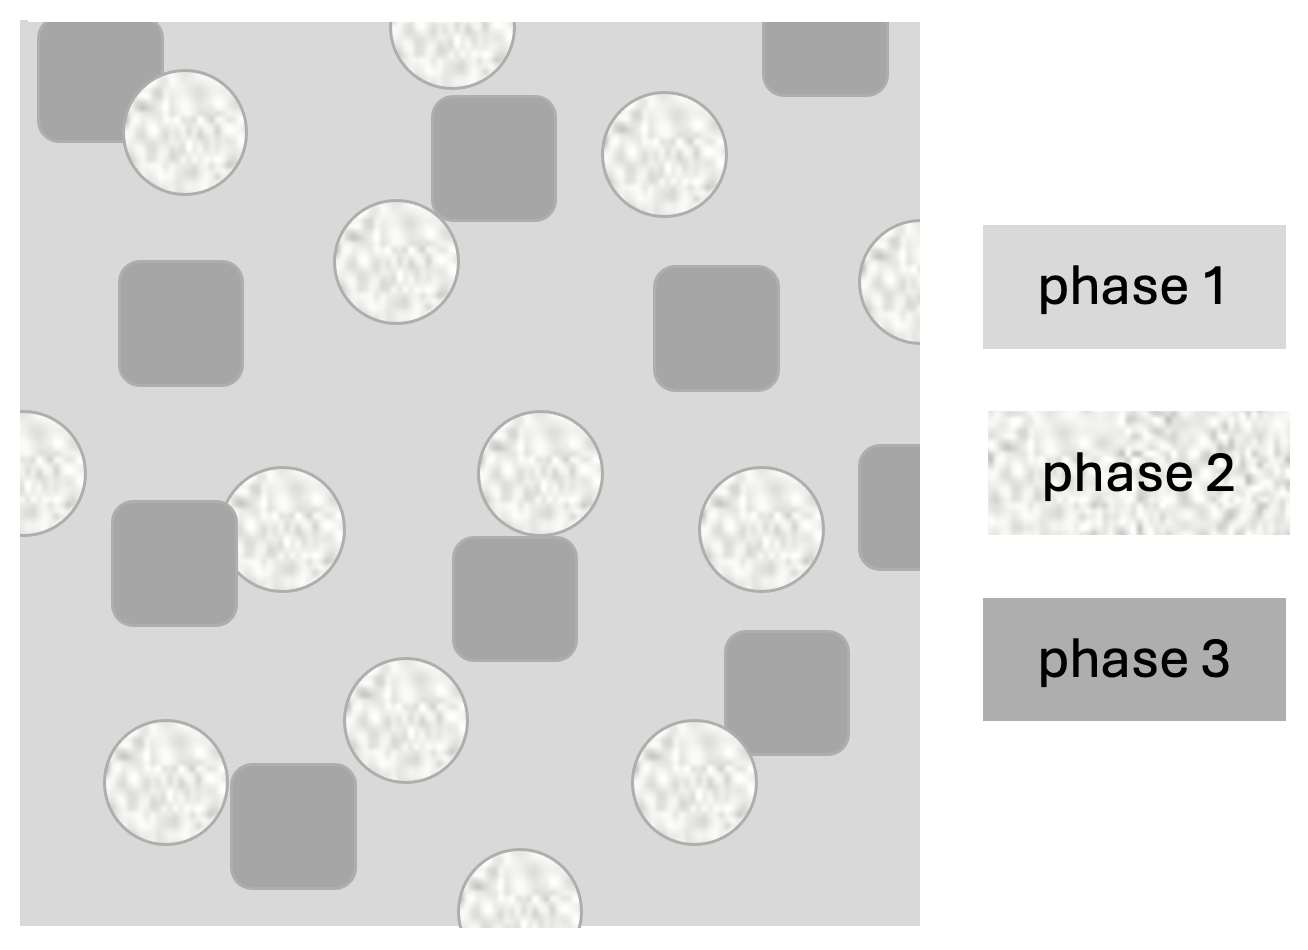
\includegraphics[width=2in,height=\textheight,keepaspectratio]{figures/3phase_composite.png}
\caption{An example of a quasi-isotropic, quasi-homogeneous 3-phase
composite. \label{fig:cartoon-3phase}}
\end{figure}

\autoref{eqn:bulk_ineq} and \autoref{eqn:shear_ineq} summarize the
results of the Hashin-Shtrikman derivations on the bounds on effective
bulk modulus \(\kappa^{*}\) and effective shear modulus \(\mu^{*}\),
where it is simultaneously required that
\(\kappa_{1} \leq \kappa_{2} \leq \dotsb \leq \kappa_{n}\) and
\(\mu_{1} \leq \mu_{2} \leq \dotsb \leq \mu_{n}\):

\begin{equation}\label{eqn:bulk_ineq}
\kappa_{1} + \frac{A_{1}^{\kappa}}{1 - \alpha_{1}^{\kappa}A_{1}^{\kappa}}
= \kappa^{*,-} \leq \kappa^{*} \leq \kappa^{*,-} = 
\kappa_{n} + \frac{A_{n}^{\kappa}}{1 - \alpha_{n}^{\kappa}A_{n}^{\kappa}}
\end{equation}

\begin{equation}\label{eqn:shear_ineq}
\mu_{1} + \frac{A_{1}^{\mu}}{1 - \alpha_{1}^{\mu}A_{1}^{\mu}}
= \mu^{*,-} \leq \mu^{*} \leq \mu^{*,-} = 
\mu_{n} + \frac{A_{n}^{\mu}}{1 - \alpha_{n}^{\mu}A_{n}^{\mu}}
\end{equation}

with \begin{equation}\label{eqn:bulk_alphas}
\alpha_{1}^{\kappa} = \frac{3}{3\kappa_{1} + 4\mu_{1}}
\quad \text{and} \quad
\alpha_{n}^{\kappa} = \frac{3}{3\kappa_{n} + 4\mu_{n}},
\end{equation}

and \begin{equation}\label{eqn:shear_alphas}
\alpha_{1}^{\mu} = \frac{3(\kappa_{1} + \mu_{1})}{5\mu_{1}(3\kappa_{1} + 4\mu_{1})}
\quad \text{and} \quad
\alpha_{n}^{\mu} = \frac{3(\kappa_{n} + \mu_{n})}{5\mu_{n}(3\kappa_{n} + 4\mu_{n})},
\end{equation}

and \begin{equation}\label{eqn:bulk_As}
A_{1}^{\kappa} = \sum\limits_{i=2}^{n} \frac{v_{i}}{\frac{1}{\kappa_{i} - \kappa_{1}} + \alpha_{1}^{\kappa}}
\quad \text{and} \quad
A_{n}^{\kappa} = \sum\limits_{i=1}^{n-1} \frac{v_{i}}{\frac{1}{\kappa_{i} - \kappa_{n}} + \alpha_{n}^{\kappa}}, 
\end{equation}

and \begin{equation}\label{eqn:shear_As}
A_{1}^{\mu} = \sum\limits_{i=2}^{n} \frac{v_{i}}{\frac{1}{\kappa_{i} - \kappa_{1}} + \alpha_{1}^{\mu}}
\quad \text{and} \quad
A_{n}^{\mu} = \sum\limits_{i=1}^{n-1} \frac{v_{i}}{\frac{1}{\mu_{i} - \mu_{n}} + \alpha_{n}^{\mu}}.
\end{equation}

The elastic forms for \(\{A_{i}^{\kappa}\}\) and \(\{A_{i}^{\mu}\}\)
differ from the general forms \(\{A_{i}\}\) because of their coupling
via the Kirchoff-St.~Venant constitutive law.

Once upper and lower bounds on the effective composite properties have
been obtained, what remains is to find a final estimate of the resulting
material properties. By the definition of bounds, we can write an
expression for the effective property as
\begin{equation}\label{eqn:mixing-param}
y^{*} = \gamma y^{*,-} + (1-\gamma) y^{*,+}.
\end{equation}

Given experimental data, one could fit \(\gamma\) and extrapolate for a
range of volume fractions, but, in the absence of experimental data, the
authors select \(\gamma = 0.5\). For more information, the reader is
referred to {[}@zohdi-course-reader{]}.

\subsection{Quantifying distributed loads with concentration
tensors}\label{quantifying-distributed-loads-with-concentration-tensors}

In addition to finding effective properties of potential composites,
\texttt{hashin\_shtrikman\_mp} recommends composites that are less prone
to failure under extreme loading. When loads are not efficiently shared
between constituents of the composite, stress concentrations, hot spots,
and electrical shorts can develop, eventually leading to material
failure. By introducing the concept of ``concentration tensors'', we can
quantify a constituent's contribution to load response and then use
constitutive laws to determine how the composite will respond to loads.

For the general case of a constitutive law of the form
\begin{equation}\label{eqn:gen-const-law}
\verb|tensor-valued response| = \verb|proportionality tensor| \times \verb|tensor-valued load|,
\end{equation}

over the domain \(\Omega\), we note that, by the definition of volume
fraction, the following holds:
\begin{equation}\label{eqn:by-vol-frac-load}
\langle \verb|tensor-valued load| \rangle_{\Omega} = \sum\limits_{i=1}^{n} v_{i} \langle \verb|tensor-valued load| \rangle_{\Omega_{i}}
\end{equation}

and \begin{equation}\label{eqn:by-vol-frac-resp}
\langle \verb|tensor-valued response| \rangle_{\Omega} = \sum\limits_{i=1}^{n} v_{i} \langle \verb|tensor-valued response| \rangle_{\Omega_{i}},
\end{equation}

where
\(\langle \cdot \rangle_{\Omega} = \frac{1}{|\Omega|} \int_{\Omega} (\cdot) \,d\Omega\)
is the average of \((\cdot)\) over the domain, \(v_{i}\) is the volume
fraction of phase \(i\), and \(n\) is the number of phases. From there,
we define the concentration tensors for the applied loads and responses
for phases \(i\in[1,...,n]\), respectively, as
\begin{equation}\label{eqn:Cload-basic-def}
\langle \verb|tensor-valued load| \rangle_{\Omega_{i}} \equiv C_{i, \text{load}} \langle \verb|tensor-valued load| \rangle_{\Omega}
\end{equation}

and \begin{equation}\label{eqn:Cresp-basic-def}
\langle \verb|tensor-valued response| \rangle_{\Omega_{i}} \equiv C_{i, \text{response}} \langle \verb|tensor-valued response| \rangle_{\Omega}.
\end{equation}

It follows from these definitions, and the assumption that the composite
is isotropic and homogeneous, that the concentration tensors can be
written only in terms of proportionality tensors. The concentration
tensors for the applied loads for phases \(i\in[2,...,n]\) are
subsequently given by \begin{equation}\label{eqn:load-conc-fact}
\begin{array}{l}
\mbox{\boldmath $C$}_{i,\text{load}} = \displaystyle\frac{1}{n-1} \displaystyle\frac{1}{v_{i}} \times \\[10pt]
\hspace{16mm} [(\text{effective } \texttt{proportionality tensor}) - (\text{phase $i$ }\texttt{proportionality tensor})]: \\[10pt]
\hspace{20mm} [(\text{phase $i$ }\texttt{proportionality tensor}) - (\text{phase 1 }\texttt{proportionality tensor})]^{-1}
\end{array}
\end{equation}

and for phase 1 as \begin{equation}\label{eqn:C1load}
\mbox{\boldmath $C$}_{1,\text{load}} = \frac{1}{v_{1}} \left( 1 - \sum\limits_{i=2}^{n} v_{i} \mbox{\boldmath $C$}_{i,\text{load}} \right).
\end{equation}

The concentration tensors for the responses for phases \(i\in[2,...,n]\)
are given by \begin{equation}\label{eqn:response-conc-fact}
\mbox{\boldmath $C$}_{i,\text{response}} = (\text{phase $i$ } \verb|proportionality tensor|)\mbox{\boldmath $C$}_{i,\text{load}}(\text{effective } \verb|proportionality tensor|)^{-1}
\end{equation}

and for phase 1 as \begin{equation}\label{eqn:C1response}
\mbox{\boldmath $C$}_{1,\text{response}} = \frac{1}{v_{1}} \left( 1 - \sum\limits_{i=2}^{n} v_{i} \mbox{\boldmath $C$}_{i,\text{response}} \right).
\end{equation}

As a concrete example, consider Ohm's law, which relates the applied
electric field \(\boldsymbol{E}\) (load) to the resulting current
density \(\boldsymbol{J}\) (response) via the electrical conductivity
\(\boldsymbol{\sigma}_{e}\) (proportionality tensor), governing a
3-phase composite. The concentration tensors for current density would
be \begin{equation}\label{eqn:J_cfs}
\begin{array}{l}
\mbox{\boldmath $C$}_{1,J} = \displaystyle\frac{1}{v_{1}} \left( 1 - v_{2} \mbox{\boldmath $C$}_{2,J} - v_{3} \mbox{\boldmath $C$}_{3,J} \right), \\[10pt]
\mbox{\boldmath $C$}_{2,J} = \mbox{\boldmath $\sigma$}_{2,e}:\mbox{\boldmath $C$}_{2,E}:(\mbox{\boldmath $\sigma$}_{e}^{*})^{-1}, \\[10pt]
\mbox{\boldmath $C$}_{3,J} = \mbox{\boldmath $\sigma$}_{3,e}:\mbox{\boldmath $C$}_{3,E}:(\mbox{\boldmath $\sigma$}_{e}^{*})^{-1},
\end{array}
\end{equation}

where \(\boldsymbol{\sigma}_{e}^{*}\) would be found according to the
previous section. The concentration tensors for electric field would be
\begin{equation}\label{eqn:E_cfs}
\begin{array}{l}
\mbox{\boldmath $C$}_{1,E} = \displaystyle\frac{1}{v_{1}} \left( 1 - v_{2} \mbox{\boldmath $C$}_{2,E} - v_{3} \mbox{\boldmath $C$}_{3,E} \right), \\[10pt]
\mbox{\boldmath $C$}_{2,E} = \displaystyle\frac{1}{2}\displaystyle\frac{1}{v_{2}} (\mbox{\boldmath $\sigma$}_{e}^{*} - \mbox{\boldmath $\sigma$}_{1,e}):(\mbox{\boldmath $\sigma$}_{2,e}^{*} - \mbox{\boldmath $\sigma$}_{1,e})^{-1}, \\[10pt]
\mbox{\boldmath $C$}_{3,E} = \displaystyle\frac{1}{2}\displaystyle\frac{1}{v_{3}} (\mbox{\boldmath $\sigma$}_{e}^{*} - \mbox{\boldmath $\sigma$}_{1,e}):(\mbox{\boldmath $\sigma$}_{3,e}^{*} - \mbox{\boldmath $\sigma$}_{1,e})^{-1}.
\end{array}
\end{equation}

In the case where the constitutive law governing concentration tensors
is the Kirchoff-St.~Venant law, which relates the tensor-valued strain
to the tensor-valued stress via the tensor-valued stiffness, we can
additionally define scalar-valued concentration factors \(C_{i,\kappa}\)
and \(C_{i,\mu}\), which respectively are the concentration factors for
hydrostatic and deviatoric stress. For phases \(i\in[2,...,n]\) They are
defined as \begin{equation}\label{eqn:sph-conc-fact}
C_{i,\kappa} = \frac{1}{v_{i}}\frac{\kappa_{i}}{\kappa^{*}}(\kappa^{*} - \kappa_{1})(\kappa_{i} - \kappa_{1})^{-1}
\end{equation}

and \begin{equation}\label{eqn:dev-conc-fact}
C_{i,\mu} = \frac{1}{v_{i}}\frac{\mu_{i}}{\mu^{*}}(\mu^{*} - \mu_{1})(\mu_{i} - \mu_{1})^{-1},
\end{equation}

where \begin{equation}\label{eqn:sph-conc-fact-def}
\left\langle \frac{1}{3}\text{tr}\mbox{\boldmath $\sigma$}\right\rangle_{\Omega_{i}} \equiv C_{i,\kappa} \left\langle \frac{1}{3}\text{tr}\mbox{\boldmath $\sigma$}\right\rangle_{\Omega} 
\end{equation}

and \begin{equation}\label{eqn:dev-conc-fact-def}
\left\langle \mbox{\boldmath $\sigma$}' \right\rangle_{\Omega_{i}} \equiv C_{i,\kappa} \left\langle \mbox{\boldmath $\sigma$}' \right\rangle_{\Omega}.
\end{equation}

For phase 1, the concentration tensors are defined as
\begin{equation}\label{eqn:sph-cf-1}
C_{1,\kappa} = \frac{1}{v_{1}} \left( 1 - \sum\limits_{i=2}^{n} v_{i} C_{i,\kappa} \right)
\end{equation}

and \begin{equation}\label{eqn:dev-cf-1}
C_{1,\mu} = \frac{1}{v_{1}} \left( 1 - \sum\limits_{i=2}^{n} v_{i} C_{i,\mu} \right).
\end{equation}

For more information, the reader is referred to
{[}@zohdi-course-reader{]}.

\section{Package overview}\label{package-overview}

\subsection{Implementation notes}\label{implementation-notes}

The library has been designed to handle the design of 2- to 10-phase
isotropic and homogeneous composites. All materials in the Materials
Project database are available for search through
\texttt{hashin\_shtrikman\_mp}, but it is recommended that users
restrict the search bounds for universal anisotropy to be between 0.5
and 1.5 for results closer to theory. Additionally, at the time of this
writing, because of the assumption that the composite and its
constituents are isotropic and homogeneous, the full tensor forms for
the effective properties and concentration tensors are collapsed to
scalar forms. This is simpler computationally and allows the same code
to be used for all properties (aside from bulk and shear moduli, which
cannot be decoupled). For material properties in the Materials Project
database with full tensor values available,
\texttt{hashin\_shtrikman\_mp} uses the largest eigenvalue.
\autoref{fig:flow-chart} is a flow chart demonstrating the most common
usage of \texttt{hashin\_shtrikman\_mp}.

\begin{figure}
\centering
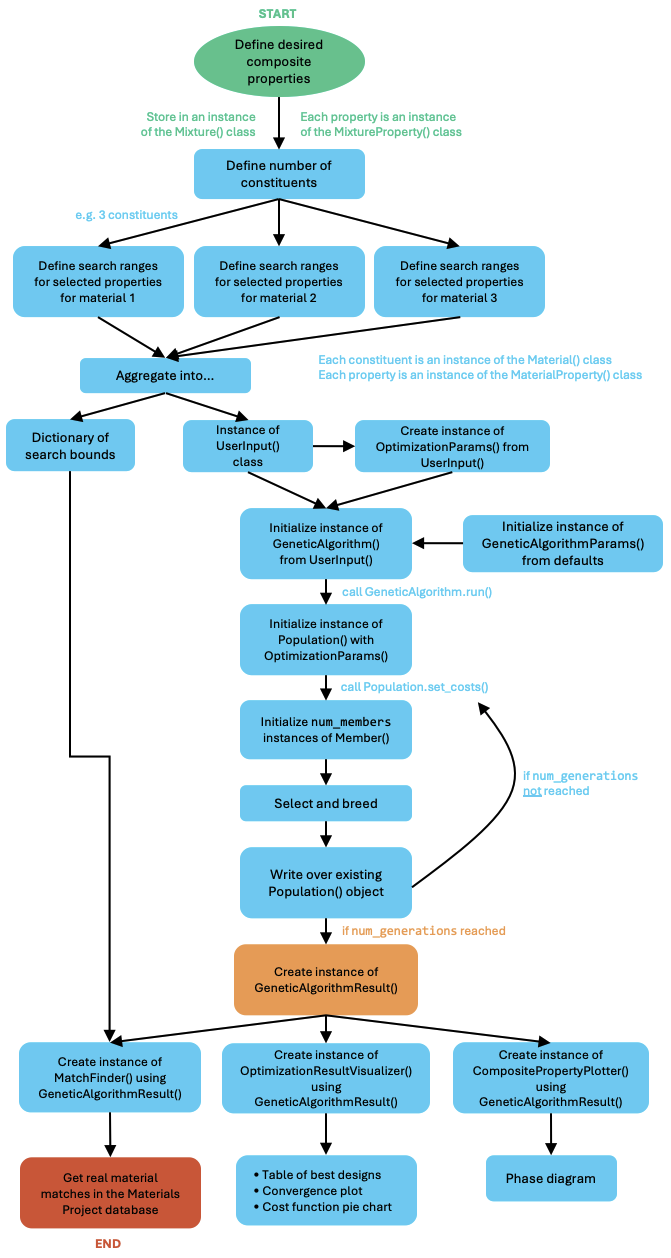
\includegraphics[width=\linewidth,height=9in,keepaspectratio]{figures/hashin_shtrikman_mp_flow_chart.png}
\caption{A flow chart demonstrating the most common usage of
\(\texttt{hashin\_shtrikman\_mp}\).\label{fig:flow-chart}}
\end{figure}

\subsection{Cost function design and optimization with genetic
algorithm}\label{cost-function-design-and-optimization-with-genetic-algorithm}

To find optimal composite mixtures, \texttt{hashin\_shtrikman\_mp}
simultaneously seeks composite compositions with effective properties
close to the desired properties and seeks to ensure even load sharing
among the composite constituent phases. Accordingly, the cost function
is constructed in the following way.

Each property category selected by a user contributes its own term to
the total cost function. At the time of this writing, the possible
property categories are elastic, dielectric, carrier-transport,
magnetic, and piezoelectric. Combining the individual cost functions to
optimize across all design goals simultaneously yields
\begin{equation}\label{eqn:pi}
\Pi^{\text{total}} = W_{\text{domains}}\left[ \Pi^{\text{elastic}} + \Pi^{\text{dielectric}} + \Pi^{\text{carrier-transport}} + \Pi^{\text{magnetic}} + \Pi^{\text{piezoelectric}} \right]
\end{equation}

where \(W_{\text{domains}}\) normalizes for the number of active
property categories. Each property category contribution is composed of
two weighted sums: 1) one with terms for absolute error between the
effective and desired properties and 2) another for the absolute error
between the concentration factors and a tolerance \texttt{TOL} that
quantifies ``well-distributed" load sharing. That is,
\begin{equation}\label{eqn:pi-gen}
\Pi^{\text{general}} =
\begin{cases}
\begin{array}{l}
w_{\text{eff}} \sum\limits_{i=1}^{n_{\text{props}}} \biggl\vert\displaystyle\frac{y_{i}^{*,D} - y_{i}^{*}}{y^{*,D}}\biggr\vert 
+ \sum\limits_{i=1}^{n_{\text{cfs}}} \hat{w}_{\text{cf}}^{i} \biggl\vert\displaystyle\frac{C_{i}-\texttt{TOL}}{\texttt{TOL}}\biggr\vert,
\end{array} & \text{if property category active}, \\
\hspace{3mm} 0, & \text{else},
\end{cases}
\end{equation}

where the superscript \(D\) denotes the desired value,
\(n_{\text{props}}\) is the number of properties in that property
category, \(n_{\text{cfs}}\) is the number of concentration factors in
that category (typically two \(\times\) the number of properties), and
\(C_{i}\) is a general scalar-valued concentration factor from section
``Quantifying distributed loads with concentration tensors''. Note also
that \(w_{\text{eff}} = 1/n_{\text{props}}\) and

\[\hat{w}_{\text{cf}}^{i} = 
\begin{cases}
w_{\text{cf}}, & C_{i} >  \texttt{TOL}, \\
0, & \text{otherwise},
\end{cases}\]

where \(w_{\text{cfs}} = 1/(2n_{\text{props}}n_{\text{materials}})\),
except in the elastic case where
\(w_{\text{cfs}} = 1/n_{\text{props}}n_{\text{materials}}\).

As a concrete example, the dielectric contribution to the cost function
would take the form \begin{equation}\label{eqn:pi-elastic}
\Pi^{\text{dielectric}} =
\begin{cases}
\begin{array}{l}
w_{\text{eff}} \biggl\vert\displaystyle\frac{\epsilon^{*,D} - \epsilon^{*}}{\epsilon_{ij}^{*,D}}\biggr\vert \\[10pt]
\hspace{3mm} + \hat{w}_{\text{cf}}^{i, E} \biggl\vert\displaystyle\frac{C_{i,E}-\texttt{TOL}}{\texttt{TOL}}\biggr\vert, 
+ \hat{w}_{\text{cf}}^{i, E_{0}} \biggl\vert\displaystyle\frac{C_{i,E_{0}}-\texttt{TOL}}{\texttt{TOL}}\biggr\vert,
\end{array} & \text{if dielectric property category active}, \\
\hspace{3mm} 0, & \text{else},
\end{cases}
\end{equation}

where the constitutive law, in the scalar case, relates applied field
\(E_{0}\) to resulting field \(E\) via the dielectric constant
\(\epsilon\) according to \(E = \epsilon E_{0}\) and the same rules for
the weights apply as above.

With the cost function defined, \texttt{hashin\_shtrikman\_mp} converges
to an optimal solution with a genetic algorithm. Each member of a
population in the genetic algorithm is composed of candidate material
property values. After successive selection and breeding over many
generations, the genetic algorithm will converge. The default genetic
algorithm parameters are 10 parents, 10 children, 200 members per
population, and 100 generations, but a user can change them. Given the
cost function design, the cost value can be thought of as the fractional
error from the desired outcome, plus penalties for ``bad" load sharing
(should contribute 0 in the case of''good" load sharing). A user can
monitor the results of the genetic algorithm with the convergence plot,
an example of which is included in \autoref{fig:convg}.

The nature of genetic algorithms is to produce several offspring with
the same properties and costs after many generations. Thus,
\texttt{hashin\_shtrikman\_mp} presents the user with only the
\emph{unique} top performing designs in a table. For the singular
lowest-cost performer, users are presented with a breakdown of the cost,
as in \autoref{fig:cost-func-contribs}.

\subsection{Visualization and
analysis}\label{visualization-and-analysis}

\texttt{hashin\_shtrikman\_mp} provides visualization tools for the
genetic algorithm results and for matches with 2-, 3-, or 4- phases.

\autoref{fig:convg} is a convergence plot showing the value of the
genetic algorithm cost function decreasing over generations. The
monotonically decreasing staircase nature is characteristic of genetic
algorithm convergence, where the best performer may remain the best for
several generations and where several genetic strings may converge to
the same value (e.g.~when the average cost of top ten performers equals
the best cost). As the cost function has been designed to represent
absolute error from the desired properties, a cost of 1.0 represents
100\% error.

\autoref{fig:cost-func-contribs} contains a breakdown of the non-zero
cost at the end of optimization for a 3-phase material where the
properties of interest were electrical conductivity, thermal
conductivity, bulk modulus, shear modulus, and universal anisotropy. We
expect the cost function to have 31 terms in this case, as there is one
effective property term per property and there are two concentration
factor terms per property per material, except in the coupled case of
bulk and shear moduli, where there are two concentration factors per
material instead of the expected four i.e.

\begin{itemize}
\item
  5 effective properties: one for each of the properties of interest,
\item
  18 non-modulus concentration factors: one load and one response
  concentration factor for each of the 3 non-elastic properties
  (electrical conductivity, thermal conductivity, and universal
  anisotropy), and for each of the 3 phases, and
\item
  6 modulus concentration factors: one hydrostatic and one deviatoric
  concentration factor for each of the 3 phases.
\end{itemize}

\begin{figure}
\centering
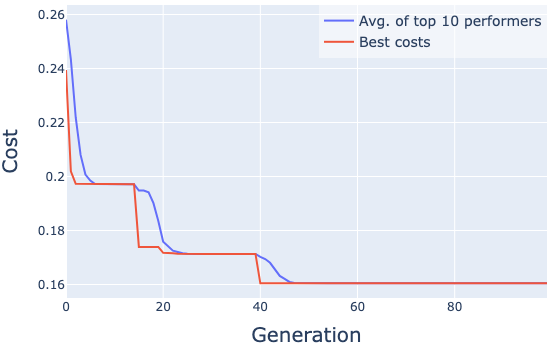
\includegraphics[width=0.6\linewidth,height=\textheight,keepaspectratio]{figures/convg.png}
\caption{An example of the convergence plot for the genetic algorithm.
\label{fig:convg}}
\end{figure}

\begin{figure}
\centering
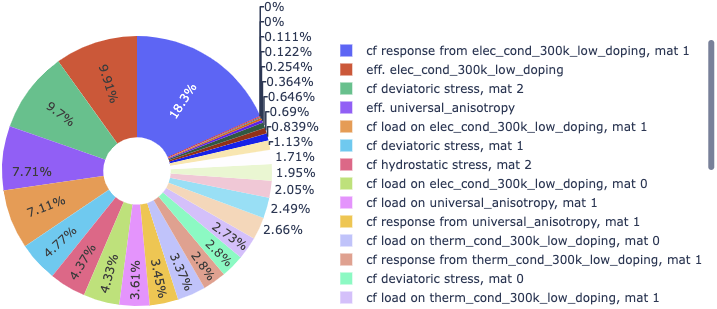
\includegraphics[width=0.9\linewidth,height=\textheight,keepaspectratio]{figures/cost-func-contribs.png}
\caption{A breakdown of the contributions to the non-zero cost at the
end of optimization. Due to the scrollable nature of the legend, only a
subset of the 31 entries is visible.\label{fig:cost-func-contribs}}
\end{figure}

Once matches have been identified for a desired composite, along with
recommended volume fractions, a user can still explore how varying the
volume fractions of the constituents affect the resulting effective
properties through interactive phase diagrams. Examples of these phase
diagrams are included in \autoref{fig:2phase}, \autoref{fig:3phase}, and
\autoref{fig:4phase}.

\begin{figure}
\centering
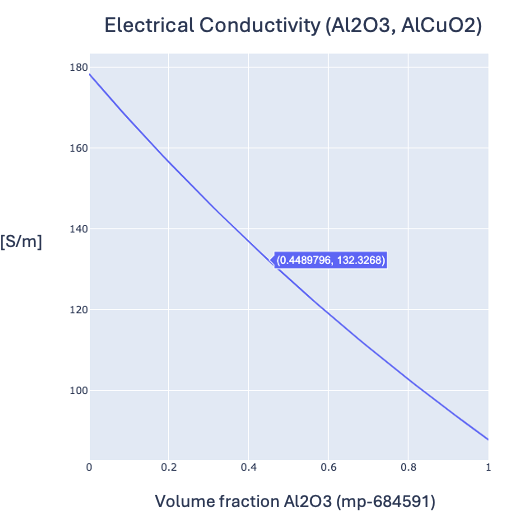
\includegraphics[width=4in,height=\textheight,keepaspectratio]{figures/elec-cond-2phase-clean.png}
\caption{Example phase diagram for a 2-phase mixture of
\(\mathrm{Al_2O_3}\) and \(\mathrm{AlCuO_2}\). The ``mp'' numbers are
the Materials Project IDs for the materials. \label{fig:2phase}}
\end{figure}

\begin{figure}
\centering
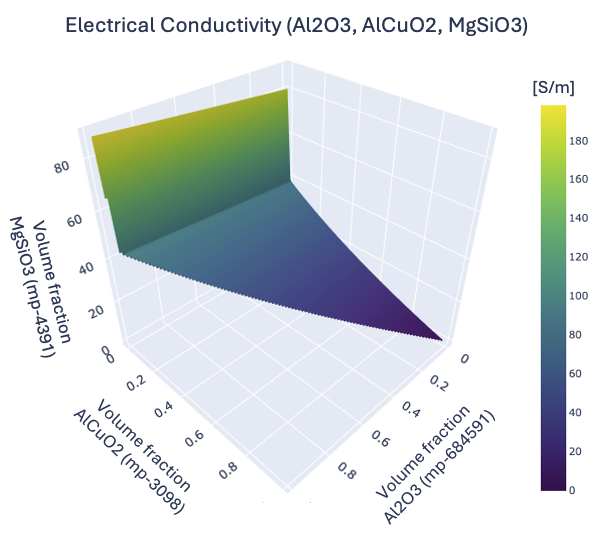
\includegraphics[width=4in,height=\textheight,keepaspectratio]{figures/elec-cond-3phase-clean.png}
\caption{Example phase diagram for a 3-phase mixture of
\(\mathrm{Al_2O_3}\), \(\mathrm{AlCuO_2}\), and \(\mathrm{MgSiO_3}\).
\label{fig:3phase}}
\end{figure}

\begin{figure}
\centering
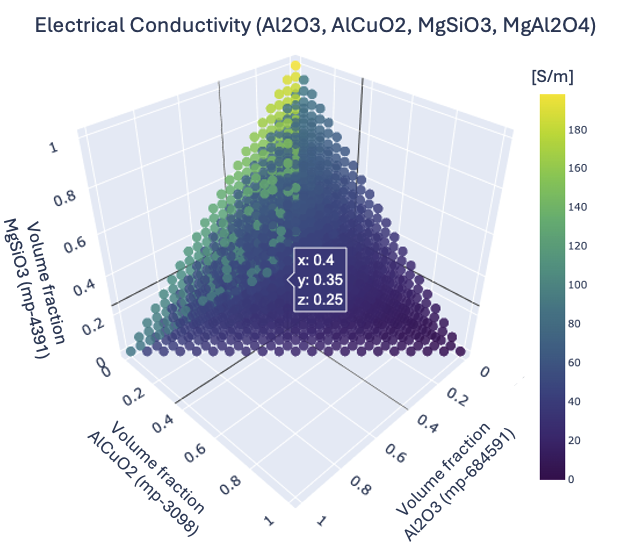
\includegraphics[width=4in,height=\textheight,keepaspectratio]{figures/elec-cond-4phase-clean.png}
\caption{Example phase diagram for a 4-phase mixture of
\(\mathrm{Al_2O_3}\), \(\mathrm{AlCuO_2}\), \(\mathrm{MgSiO_3}\) and
\(\mathrm{MgAl_2O_4}\). \label{fig:4phase}}
\end{figure}

\subsection{Match-finding}\label{match-finding}

The genetic algorithm returns suggested material properties for each of
the phases in the composite and then \texttt{hashin\_shtrikman\_mp}
finds real materials in the Materials Project database which are
similar, according to some percent error threshold, which the user can
control.

\section{Acknowledgments}\label{acknowledgments}

This work was primarily funded by the Materials Project, which is funded
by the U.S. Department of Energy, Office of Science, Office of Basic
Energy Sciences, Materials Sciences and Engineering Division, under
Contract no. DE-AC02-05-CH11231: Materials Project program KC23MP. The
project has been intellectually led by Tarek Zohdi and Kristin Persson.
We would also like to thank the software engineering team at the
Materials Project -- Patrick Huck, Jason Munro, and Ruoxi Yang -- for
their support.

\section{References}\label{references}
